\chapter{Introduction}
\label{chap:intro}

\section{Soft matter physics}\label{sec:softmatt}

Broadly speaking, the results presented in this dissertation involve those physical systems in which nontrivial collective behavior emerges from the competition among hydrophobicity, entropy, and elasticity.
These systems are a subset of the broad field of soft matter physics, also referred to as complex fluids.
In general, soft matter physics revolves around materials in which their constituents have a size in the range $10$ nm -- $1$ $\mu$m, their dynamics are mostly diffusive, and thermal fluctuations play an important role -- that is, the relevant energy scales of important physical behaviors of these systems are comparable with the thermal energy at room temperature: roughly $0.6$ kcal$\cdot$mol$^{-1}$.
I will be primarily concerned with colloids and polymers; other systems such as liquids, gels, and biological materials (such as membranes) are also included in this field.

Soft materials exhibit a number of characteristics not seen in ``hard'' condensed matter.
One of the most important is the formation of mesoscopic structures, which are intermediate in scale between the individual components (e.g. colloids or polymers) and the bulk, macroscopic system.
Soft matter systems also tend to undergo large fluctuations due to their relatively low energy density, and their most interesting equilibrium properties tend to be dominated by entropy rather than energy.
The result is that soft matter systems often exhibit unique behaviors which are difficult to predict.

An example of such complicated dynamics is in the crystallization of binary systems of hard colloids; that is, systems containing hard, purely repulsive spheres of two different sizes~\cite{FrenkelNatMat}.
Because these particles cannot overlap and interact only via their hard repulsions, the energy in such systems is by definition zero.
However, a wide range of three-dimensional crystalline structures is found, depending on the relative sizes and concentrations of the two components; these interesting effects must necessarily be due solely to the configurational entropy of the system.

Over the last fifty years, a large effort has been devoted to establishing the theoretical and numerical tools with which to characterize and predict the phase behavior of complex fluids.
Most studies have focused on systems where the effective interactions between the main components are solely dependent on the interparticle separation.
However, recent advances in synthesis of nanoparticles~\cite{DeVries,Schnablegger,Hong,Weller,Hobbie,weitz,pine,mitragotri} have allowed for unprecedented control over the  shape and surface chemistry of colloidal particles;
it has also become feasible to engineer interactions between star polymers or dendrimers by controlling their overall chemical and topological properties~\cite{mladek}.
The result is an unlimited number of potential building blocks whose organization, either from a dilute fluid by aggregation due to interparticle attractions or from a dense fluid by an externally-applied pressure, have the potential to form a large variety of structures with novel functional, mechanical, and optical properties.

\section{Self-organization}

This dissertation deals with the process by which these mesoscopic and/or the full macroscopic structures form.
The work presented is the result of Monte Carlo and molecular dynamics simulations on a wide variety of systems representing a small subset of the variety described above, directed at studying the ways in which the details of interparticle interactions affect how self-organization occurs.

This self-organization of structures can be considered as divided between two broad situations: formation of macroscopic structures, which can be modeled by classical nucleation theory, and aggregation into mesoscopic structures, which is described in the framework of self-assembly theory.

\subsection{Classical nucleation theory}\label{sec:CNT}

Although the generic features of particle aggregation can be described, at least phenomenologically, in terms of simple thermodynamic arguments~\cite{Israelachvili, Zhang, Leckband, Nagarajan, glotzer2}, the details of the self-organization process are far from being understood, even in the simple case of aggregation of isotropic particles into macroscopic three-dimensional crystals.
For more complex particles, it is difficult to predict, \textit{a priori}, the equilibrium self-assembled state, and, even more interestingly, the nonequilibrium pathways associated with it.~\cite{Hong2}.

The thermodynamics of crystal formation can be described, to a first approximation, within the framework of classical nucleation theory (CNT).
In this theory, the nucleation and eventual crystallization of a system is described as a simple interplay between two competing thermodynamic forces; however,
it includes some fairly severe approximations which make it applicable only for a qualitative understanding of the process.

Consider a system of $N$ particles interacting via some potential.
Within this system is a roughly spherical nucleus of $n$ crystalline particles surrounded by a fluid of the remaining $(N-n)$ particles (note that for small $n$, the approximation of a spherical shape is a poor one).
Figure~\ref{fig:xtal} shows an illustration of this system.
There are two major contributions to the free energy of this nucleus: the free energy gain associated with the formation of the more stable crystal phase, and the free energy cost due to the interface between the fluid and the solid phase.
Below I will focus on these two terms in more detail.
\begin{figure}
	\begin{center}
		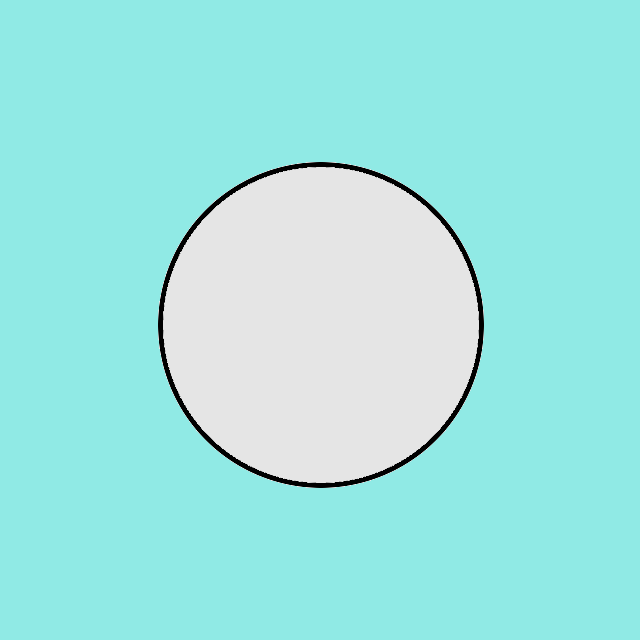
\includegraphics[width=0.4\textwidth]{xtal.png}
		\put(-117.5,80){\LARGE{Crystal}}
		\put(-110,15){\LARGE{Fluid}}
	\end{center}
	\caption[An illustration of a spherical crystal in the presence of a fluid]{An illustration of the system considered in classical nucleation theory; a spherical crystal embedded in a fluid phase.  The dark border indicates the interface.}\label{fig:xtal}
\end{figure}

%\subsection{The free energy gain due to organization}

For a typical scenario of a system of particles interacting via a short-ranged attractive potential, at sufficiently large density $\rho$, the free energy associated with the growth of the crystal is favorable because the chemical potential difference, $\Delta \mu$, between the fluid and crystalline phases becomes negative.
The condition that $\Delta \mu < 0$ is generally due to a combination of several factors; the most obvious contribution is a direct consequence of favorable interparticle energetics.
A particle in a crystal has, on average, more neighbors than one in the fluid, and thus, crystallization leads to an energy gain.
However, a favorable $\Delta \mu$ may also arise in systems featuring purely repulsive interparticle interactions, and the origin of this effect is more subtle.

For illustration, consider a system of hard spheres.
These particle interact via the potential
\begin{equation}V = \begin{cases} \infty & \textrm{if } r < r_0 \\ 0 & \textrm{otherwise}\end{cases}\,,\end{equation}
where $r$ is the distance between particles and $r_0$ is the particle diameter; therefore, as in the example system discussed in Section~\ref{sec:softmatt}, their phase bahavior is completely determined by their configurational entropy -- the interaction energy within such a system is by definition always zero.
However, very early computer simulations~\cite{Wood,Alder} showed that even these simple systems showed a transition from a fluid to a stable, face-centered cubic (fcc) crystal.

The existence of a stable crystalline phase for hard spheres implies that beyond some density $\rho$, the configurational entropy of the ordered, crystalline phase is higher than that of a disordered phase.
However, intuition and a simple consideration of the system neglecting the correlation between particles due to their excluded-volume (repulsive) interactions in the hard sphere system leads one to the conclusion that the disordered phases is higher in entropy at every density.
This indicates that excluded-volume effects must be vital for this transition, and indeed, it is clear that such effects must be important at high $\rho$.

At high enough density $\rho$, the disordered fluid phase becomes over-compressed -- the particles can no longer easily diffuse past each other and the system becomes stuck in a disordered but ``jammed'' state.
The key to understanding the existence of the crystalline state of hard spheres then is that the amount of free volume available to each particle in a fcc crystal is larger than that avilable to each particle in an over-compressed fluid.
Each particle in the crystal is therefore a bit freer to move than the particles in the disordered fluid -- and so the system has a slightly higher configurational entropy.

Thus, even in purely repulsive systems such as hard spheres, when the density $\rho$ is large enough, the free energy of crystalization, $\Delta \mu$, is negative, due to the gain in configurational entropy upon self-organization.

This negative $\Delta \mu$ results in a linear decrease of the Gibbs free energy with the number of crystalline particles in the interior of the nucleus; for large-enough spherical nuclei, it is approximately
\begin{equation}\Delta G_{\mu} (r) \simeq \frac{4}{3} \pi r^3 \rho \Delta \mu \,,\end{equation}
where $r$ is the radius of the nucleus and $\rho$ is the crystal density.
The chemical potential difference $\Delta\mu$ can easily be determined numerically; however, what is important for this qualitative understanding of classical nucleation is that in order for crystal nucleation to occur, $\Delta \mu$ must be negative.

%\subsection{Interfacial free energy}

The second major term in the full free energetic description of crystal nucleation is the free energy cost associated with the creation of an interface between the crystal nucleus and the fluid phase.
One can think of this term as arising from the loss of entropy of a particle bound to the surface versus one in the fluid, without benefit of a full complement of favorable interactions with neighbors (for attractive particles) or the full configurational entropy gain of increased free volume (for purely repulsive ones) experienced by a particle in the interior.
It is described by the surface tension $\gamma$, a quantity the value of which, like $\Delta \mu$, is unimportant for our purposes except that it must be positive.
The interfacial free energy is then the product of the surface area times the surface tension
\begin{equation}\Delta G_{\gamma} (r) = A \gamma = 4 \pi r^2 \gamma \,.\end{equation}

%\subsection{Consequences and limitations of CNT}
We thus find the total Gibbs free energy of the crystal nucleus, as a function of the nucleus size $r$,
\begin{equation}\Delta G \simeq \frac{4}{3} \pi r^3 \rho \Delta \mu + 4 \pi r^2 \gamma \,.\end{equation}
Taking the derivative of this quantity and setting the result equal to zero, a local maximum in the free energy is located at
\begin{equation}r^* \simeq \frac{2 \gamma}{\rho \left|\Delta \mu \right|} \,,\end{equation}
or, in terms of the number of particles in the cluster,
\begin{equation}n^* \simeq V_c \rho \simeq \frac{4}{3} \pi \left(r^*\right)^3 \rho \simeq \frac{32 \pi}{3 \rho}\left(\frac{\gamma}{\left|\Delta \mu\right|}\right)^3\,\,\,.\end{equation}

This is termed the ``critical nucleus size'', and represents a transition point: $50\%$ of particles of size $r^*$ would be expected to melt back to the fluid phase, and $50\%$ would be expected to grow into very large crystals.
In fact, in this approximation, nuclei larger than $r^*$ would be expected to grow until they included every particle in the system.

\begin{figure}
	\begin{center}
		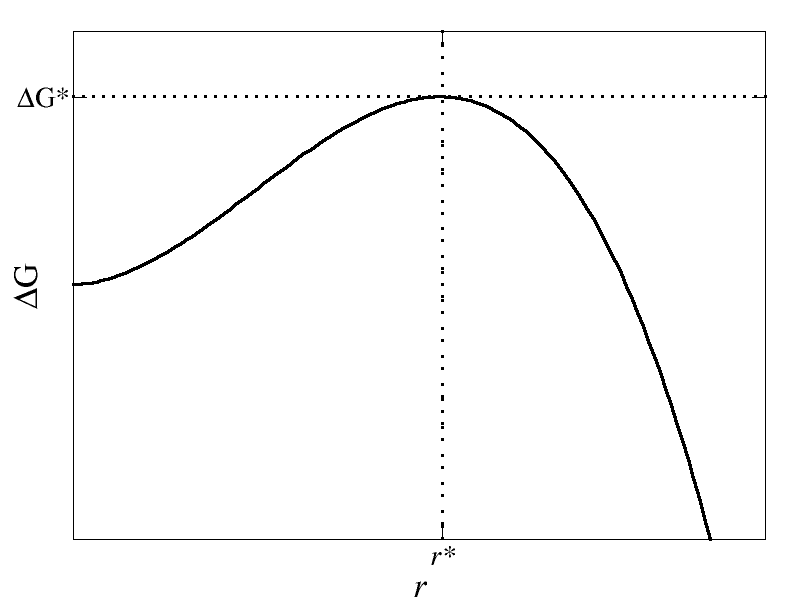
\includegraphics[width=0.6\textwidth]{CNT.png}
	\end{center}
	\caption[$\Delta G$ vs. $r$ in classical nucleation theory]{A plot of $\Delta G$ vs. $r$ for a crystal nucleus surrounded by a fluid.  The critical nucleus is at the point where the dotted lines, indicating $\Delta G^*$ and $r^*$, cross.}\label{fig:CNT}
\end{figure}

Plugging the critical radius $r^*$ into the expression for $\Delta G$ derived above yields the free energy cost of the critical nucleus,
\begin{equation}\Delta G^* \simeq \frac{16 \pi \gamma^3}{\rho^2 \Delta \mu^2}\,.\label{eq:dGCNT}\end{equation}
An illustration of the form of this free energy landscape is plotted in Figure~\ref{fig:CNT}.

In order for large, crystalline aggregates to form via classical nucleation, a balance must be achieved in $\Delta G^*$; because the rate of crystal nucleation $\tau \propto e^{-\beta \Delta G^*}$ (where $\beta \equiv \left(k_{\textrm {B}}T\right)^{-1}$), if it is too large, a critical nucleus will not be observed over experimentally relevant timescales, and thus the barrier will never be crossed in practice.
However, if $\Delta G^*$ is too small, several critical nuclei will occur throughout the system.
While it may be possible for these disparate nuclei to coalesce into a single large crystalline cluster, the segregation of the system into several small clusters can make it more difficult for a large cluster to form.

In general, the handles by which we can affect $\Delta G^*$, as expressed in equation~\ref{eq:dGCNT}, are indirect and through $\Delta \mu$ and $\gamma$ -- in particular, their values will depend on the temperature and concentration of the surrounding fluid, and these parameters can in principle be adjusted by altering the position in $\rho-T$ phase space so that $\Delta G^*$ will have some ``optimal'' value at which one crystal will form on an experimentally-accessible time scale.
Chapter~\ref{chap:pixel} explores other methods for adjusting $\Delta G^*$.

Finally, a comment regarding the problems with the approximations involved with CNT.
As briefly mentioned above, the assumption of a spherical nucleus breaks down for small nuclei; furthermore, the substitution of $n = \frac{4}{3} \pi r^3 \rho$ relies on the nucleus being large and homogeneous, and the surface tension $\gamma$ may have a weak dependence on the curvature of the surface and thus the size of the nucleus.

One last important assumption that is made in CNT and is not necessarily valid for any system is that the symmetry of the crystalline nucleus is the equilibrium structure of the final macroscopic crystal.
For example, the equilibrium structure of a crystalline hard sphere system is fcc; however, during the nucleation process, the forming nucleus contains other crystal structures; particularly, a not-insignificant fraction of hexagonal close-packed (hcp) defects, in a structure referred to as random-stacked close-packed (rhcp)~\cite{auerthesis}.

\subsection{Self-assembly and the critical micellar concentration}\label{sec:cmc}
Classical nucleation theory deals with the formation of macroscopic crystals from a fluid phase; when systems form several finite-sized mesoscopic structures, a different theoretical framework becomes more appropriate.
Several biological structures are formed in this way, including viral capsids and biological membranes.

For example, biological membranes are formed by self-assembly of lipids: amphiphilic molecules with hydrophilic head groups and hydrophobic tails consisting of hydrocarbon chains.
When these molecules are placed in water, the hydrocarbon tails will aggregate together due to their hydrophobicity, forming specific structures.

Amphiphilic molecules tend to be shaped roughly like a truncated cone, with the hydrophilic head group representing the base of the cone and the hydrocarbon tails representing the tip -- thus, when they self-assemble, they can form various shapes depending on their aspect ratio, $\xi = \frac{V}{ah}$, where $V$, $a$, and $h$ are the volume, base area, and height of this cone, respectively.
When $\xi = \frac{1}{3}$ (a cone) the equilibrium structure is a sphere, and when $\xi =1$ (a cylinder), a lamellar, planar structure is formed.  These lamellar structures can then stack, with their hydrophobic surface facing each other, to form planar bilayers.
When $\xi$ is slightly less than $1$, these bilayers curve and can loop back on themselves, forming vesicles with hydrophobic surfaces on both the exterior and interior; value of $\xi$ between $\frac{1}{3}$ and $1$ form various non-spherical micelles.

Self-assembly of micellar structures sets in at a defined concentration of monomers known as the critical micellar concentration (cmc), $c^*$.
It can be approximately calculated as follows.

Consider a system of $N$ lipids in a volume $V$.
They self-assemble into aggregates of size $\alpha$, defined as the number of molecules in the aggregate; the number of molecules in aggregates of size $\alpha$ is $N_\alpha$, and the number of such aggregates is $n_\alpha = \frac{N_\alpha}{\alpha}$.
The partition function for non-interacting micelles is given by
\begin{equation}
Q^{\textrm {(id)}} = \prod_{\alpha = 1}{N} \frac{1}{n_\alpha!} \left(\frac{V q_\alpha^{\textrm {int}}}{\Lambda_\alpha^3}\right)^{n_\alpha} \,,
\end{equation}
where $q_\alpha^{\textrm {int}}$ is the internal partition function of an aggregate of size $\alpha$.
Given this, the chemical potential per lipid molecule in an aggregate of size $\alpha$ is
\begin{equation}
\mu_\alpha = \frac{k_{\textrm B} T}{\alpha} \ln\left(\frac{x_\alpha}{\alpha}\right) + \epsilon_\alpha \,,
\end{equation}
where $x_\alpha = \frac{N_\alpha}{N}$ is the mole fraction of the lipids that belong to aggregates of size $\alpha$ and $\epsilon_\alpha = -\frac{k_{\textrm B}T}{\alpha}\ln \left(\frac{q_\alpha^{\textrm {int}} v}{\lambda_\alpha^3}\right)$, where $v$ is the volume per lipid molecule.

If all aggregates are in equilibrium, then all of these chemical potentials are equal, $\mu_\alpha = \mu$ for all $\alpha$.
Then
\begin{equation}
x_{\alpha} = \alpha x_1^\alpha e^{(\alpha(\epsilon_1-\epsilon_\alpha)/k_{\textrm B}T)} \,,\label{cmc1}
\end{equation}
where $k_{\textrm {B}}$ is the Boltzmann constant ($k_{\textrm {B}} \simeq 1.38 \times 10^{-23} \textrm{J} \cdot \textrm{K}^{-1}$) and $T$ is the system temperature.

The cmc, $x_c$, is defined as the mole fraction at which the total mole fraction of aggregates with $\alpha \geq 2$ is equal to $x_1$,
\begin{equation}\sum_{\alpha \geq 2} x_\alpha = x - x_1 = x_1\,.\end{equation}
If the geometry of the lipids is such that a micelle of a specific size $\alpha^*$ is favored, then $\epsilon_\alpha$ will have a minimum at that value $\alpha = \alpha^*$, so that $\frac{\partial \epsilon_{\alpha^*}}{\partial \alpha} = 0$.
\begin{equation}\sum_{\alpha \geq 2} x_\alpha \simeq x_{\alpha^*} = x_1 = \frac{x_c}{2}\,.\label{cmc2}\end{equation}
Subsituting Equation~\ref{cmc1} into Equation~\ref{cmc2} yields an expression for the cmc,
\begin{equation}
	x_c \simeq 2 e^{\beta(\epsilon_{\alpha^*}-\epsilon_1)} \,. 
\end{equation}
This is the approximate mole fraction at which half of the lipid molecules in the system are members of an aggegrate of size $\alpha^*$.

It is important to note that the calculation of the cmc considers only thermodynamic factors, and does not consider kinetic ones at all.
If most of the particles in the system are members of aggregates, the primary process by which large aggregates form from smaller ones is Ostwald ripening,
which requires the dissolution of a smaller aggregate followed by the deposition of its component particles on the surfaces of others.

However, if the equilibrium aggregate size is $\alpha^*$, there will be some range of aggregate sizes smaller than $\alpha^*$ for which the free energy of the aggregates is lower than the free energy of individual particles.
Thus, the dissolution of these aggregates incurs a free energetic penalty; it is possible for the system to become trapped in a metastable state in which some or all of the aggregates in the system are smaller than the equilibrium size $\alpha^*$, because these aggregates will not dissolve to allow for the growth of others over experimentally accessible timescales.

\section{Exploring ``anisotropy space''}\label{sec:anisotropy}
Whether we are considering aggregation of particles into macroscopic three-dimensional crystals or finite-sized clusters, the shape and the interaction patterns between the single components greatly affects the structure of the final aggregates.

The advances in particle synthesis mentioned above have led to the opening of a vast, multidimensional space of particle anisotropy.
In order to fully explore the possibilities for self-organization in this new space, exploration outside of the traditional $\rho-T$ phase diagram is required.
Following \citeauthor{glotzer}~\cite{glotzer}, I will refer to this multidimensional phase space as ``anisotropy space''.

Every chapter of this dissertation, and indeed much of the work in the field of soft matter physics, can be thought of as exploration along one or more axes in anisotropy space.
For example, in Chapter~\ref{chap:janus}, we explore the axis of degree of hydrophobicity in a system of asymmetric Janus particle, from 0\% (purely repulsive spheres) to 100\% (particles with an isotropic attractive potential).
In Chapter~\ref{chap:aspherical}, we introduce two anisotropy axes, labeled $A$ and $q$, which allow us to characterize aspherical particles with respect to purely isotropic hard spheres.

Most work in this field involves exploration of of the forward self-organization problem; that is, one or more axes of anisotropy are chosen, and the effect of that anisotropy on the behavior of systems of those particles is determined.
Chapter~\ref{chap:pixel} attempts to address the reverse problem: given a defined set of anisotropy axes (in this case, interaction energy and patch size), this work attempts to find the region or regions in phase space which will yield desired system behavior, such as self-organization into a specified target structure.

In principle, anisotropy space is infinite; even the region of anisotropy space accessible by current particle synthesis methods (or found in nature) is very large.
Thus, an important part of the challenge in exploring this space is identifying which regions of the space are both experimentally accessible and likely to yield nontrivial results.
In the case of this dissertation, ``nontrivial results'' generally means crystallization that in some way differs (for example, in thermodynamics, mechanism, or crystal structure) from that of the relevant isotropic reference -- most often, some approximation of a hard sphere.

\begin{figure}	
	\begin{center}
		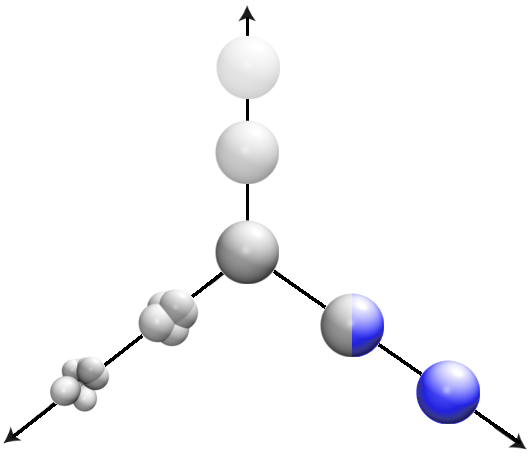
\includegraphics[width=0.6\textwidth]{anisotropyspace.png}
		\put(-133,212){(c)}
		\put(-260,22){(b)}
		\put(-15,20){(a)}
	\end{center}
	\caption[Anisotropy space]{An illustrated example of anisotropy space, with a hard sphere as the origin (``zero anisotropy'') and axes of (a) degree of hydrophobicity (Chapter~\ref{chap:janus}), (b) asphericity (Chapter~\ref{chap:aspherical}), and (c) softness (Chapter~\ref{chap:2dsoft}) (figure adapted from \citeauthor{glotzer}~\cite{glotzer}).}
\end{figure}


\section{Frequently-used numerical methods}
In this section, I will briefly describe two methods that are used frequently throughout this work.
First, a method by which crystalline order can be differentiated from the surrounding fluid will be discussed; next, an algorithm for calculating free energy differences with respect to a reference state is demonstrated.

\subsection{Measuring crystalline order using spherical harmonics: $\bar {\bf q}_l$}\label{sec:orderparamdesc}

The crystallinity of a system can be measured quantitatively using a local bond-order parameter originally introduced by Steinhardt \textit{et al.}~\cite{ronchetti} and used, for example, in~\cite{tenwolde,auer} and many others.
This method uses $l$-fold symmetric spherical harmonics to numerically differentiate crystal structures of that symmetry (most commonly, $l=6$, so that body-centered cubic [bcc], fcc, or hcp structures are detected) from the fluid.

For a given particle $i$, we define $q_l(i)$ as follows:
\begin{equation}
	q_l(i) = \left(\frac{4 \pi}{13} \sum_{m=-l}^{l} \left| q_{lm}(i) \right|^2\right)^{1/2} \,,
\end{equation}
where
\begin{equation}
	q_{lm}(i) = \frac{1}{N_b(i)} \sum_{j=1}^{N_b(i)}Y_{lm}\left(\hat{\bf r}_{ij}\right) \,.
\end{equation}
The sum in this equation is over all neighboring particles $j$ of particle $i$, where a particle is defined as ``neighboring'' if it is within some cutoff $r_q$ of particle $i$; $N_b(i)$ is the number of such neighboring particles to particle $i$.
$Y_{lm}\left(\hat{\bf r}_{ij}\right)$ is the $m$-component spherical harmonic evaluated for the normalized vector $\hat{\bf r}_{ij}$ from particle $i$ to particle $j$.

This parameter, $q_l(i)$, is sensitive to the degree of orientational correlations between vectors joining neighboring particles -- in a fluid, there are no preferred orientations and so the correlations decay rapidly, whereas in a crystal, the vectors are strongly correlated.
We can thus calculate a quantitative measure of the degree of crystallinity, and define two particles as ``connected'' within a crystalline structure if the correlation between neighboring particles,
\begin{equation}
	{\bf q}_l(i)\cdot{\bf q}_l(j) = \sum_{m=-l}^l q_{lm}(i) \cdot q_{lm}^*(j) \,,
	\label{eq:orderparam}
\end{equation}
is greater than some cutoff value $q_{\textrm {cut}}$.
Alternatively, the values of ${\bf q}_l(i) \cdot {\bf q}_l(j)$ can be averaged, for each particle $i$, over all neighbors $j$, yielding a single value $\bar q_l(i)$ -- comparing the result to a cutoff $q_{\textrm {cut}}$ allows particle $i$ to be defined as ``crystalline'' or ``non-crystalline.''
The number of connected particles to particle $i$ is denoted $N_X(i)$.
Figure~\ref{fig:q6dist} shows distributions of $q_6$, $q_4$, and $N_X$ values in liquid, bcc, and fcc systems, in order to illustrate the power of these measures for delineating crystalline vs. noncrystalline systems.

\begin{figure}
	\begin{center}
		\subfloat[]{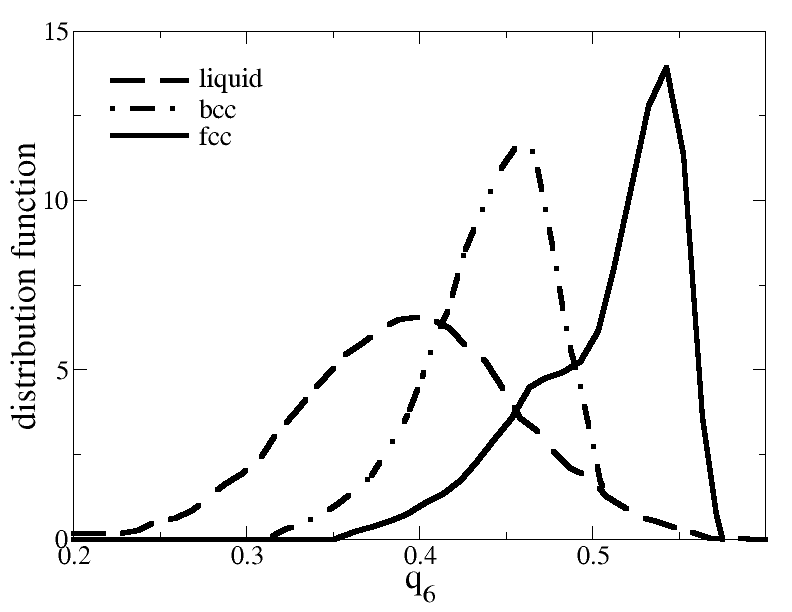
\includegraphics[width=0.6\textwidth]{q61.png}\label{q61dist}}

		\subfloat[]{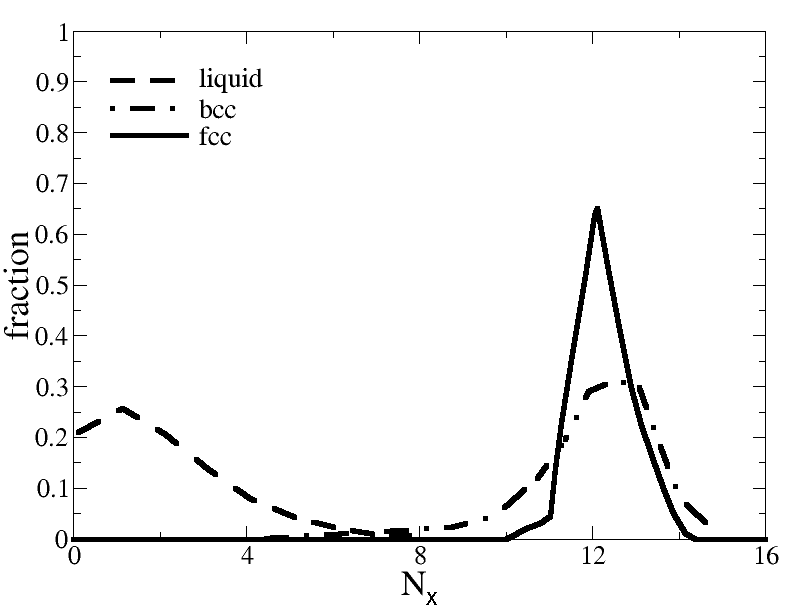
\includegraphics[width=0.6\textwidth]{q62.png}\label{q62dist}}
	\end{center}
	\caption[The distribution of $q_6$ and $N_X$ for liquid, bcc, and fcc systems]{The distribution of~\subref{q61dist} $q_6$ and~\subref{q62dist} $N_X$ for liquid, bcc, and fcc systems (figures created from data in \citeauthor{tenwolde2}~\cite{tenwolde2}).  While the $q_6$ values are different for the three systems, note that the number of connections $N_X$ is the strongest distinguisher between crystalline and noncrystalline systems, due to the fact that it accounts for relative orientation between neighboring particles.}\label{fig:q6dist}
\end{figure}

This order parameter will be used extensively throughout this dissertation.
In most cases, the six-fold symmetric $q_6$ will be used; in Chapter~\ref{chap:pixel}, $q_4$ is used, and some comments will be presented on the use of $q_4$ and $q_6$ values to differentiate between crystals of four- and six-fold symmetry.

\subsection{Calculating free energies: thermodynamic integration}\label{sec:thermint}
It is often desirable to compute the free energy of a system with respect to some reference.
One method for doing so, and the one that will be used in this dissertation (particularly, Chapter~\ref{chap:brush}), is thermodynamic integration~\cite{FrenkelBook}.

The Helmholtz free energy, $F$, is related to the canonical partition function $Q$ as follows:
\begin{align}	
	F &= - k_{\textrm B} T \ln Q(N, V, T) \notag \\
	&\equiv -k_{\textrm B} T \ln \left(\frac{\int d {\bf{p}}^N d {\bf{r}}^N \exp\left[-\beta \mathcal{H}({\bf {p}}^N, {\bf {r}}^N)\right]}{\Lambda^{dN} N!}\right) \,,
\end{align}
where $\mathcal{H}$ is the Hamiltonian of the system; $\bf p$ and $\bf r$ are the momenta and positions of all particles in the system, respectively; $d$ is the dimensionality; $N$ is the number of particles; $V$ is the volume; $T$ is the temperature; and the thermal de Broglie wavelength $\Lambda \equiv \frac{h}{\sqrt{2 \pi m k_{\textrm B} T}}$.

Assume that we can write the potential energy in a three-dimensional system, $V_\lambda$, as a linear function of some coupling parameter $\lambda$, such that for $\lambda = 0$, $V_\lambda$ equals some reference potential $V_{\textrm {ref}}$, and for $\lambda = 1$, $V_\lambda$ equals the potential of interest $V$:
\begin{equation}
	V_\lambda = (1 - \lambda)V_{\textrm {ref}} + \lambda V = V_{\textrm {ref}} + \lambda(V - V_{\textrm {ref}}) \,.
\end{equation}

Then, for a given value of lambda, the partition function $Q(N, V, T, \lambda)$ is given by
\begin{equation}	
	Q(N, V, T; \lambda) = \frac{1}{\Lambda^{3 N} N!}\int{d {\bf {r}}^N e^{-\beta V_\lambda}} \,.
\end{equation}
The derivative of $F$ with respect to $\lambda$ can then be written
\begin{align}
	\left(\frac{\partial F(\lambda)}{\partial \lambda}\right)_{N, V, T} &= -\frac{1}{\beta} \frac{\partial}{\partial \lambda} \ln Q(N, V, T; \lambda) \notag\\
	%&= -\frac{1}{\beta Q(N, V, T, \lambda)} \frac{\partial Q(N, V, T, \lambda)}{\partial \lambda} \notag\\
	&= \frac{\int{d {\bf {r}}^N \left(\frac{\partial V_{\lambda}}{\partial \lambda}\right)e^{-\beta V_\lambda}}}{\int{d {\bf {r}}^N e^{-\beta V_\lambda}}} \notag\\
	&\equiv \left<\frac{\partial V_\lambda}{\partial \lambda}\right>_\lambda \,,
\end{align}
where the notation $\left<...\right>_\lambda$ is used to denote the ensemble average for a system with potential energy function $V_\lambda$.

The energy difference between the system with the potential of interest $V$ and the reference system with potential $V_{\textrm {ref}}$ can then be found by integrating
\begin{equation}
	\Delta F \equiv F(\lambda = 1) - F(\lambda = 0) = \int_{\lambda = 0}^{\lambda = 1} d\lambda \left<\frac{\partial V_\lambda}{\partial \lambda}\right>_\lambda \,. \label{deltaF}
\end{equation}
Thus, the free energy difference $\Delta F$ can be calculated by integrating a derivative of the readily accessible quantity, the total potential, with respect to $\lambda$.
In practice, this is done by sampling at several values of $\lambda \in \left[0,1\right]$ and integrating numerically.

\section{Organization of this dissertation}

This dissertation is organized as follows.

In Chapter~\ref{chap:janus}, we discuss the self-assembly of particles with partially hydrophobic and partially hydrophilic surfaces, and determine the effect of the ratio of the two areas.
It is based on work published in~\cite{cacciuto}.


Chapter~\ref{chap:aspherical} presents studies of the thermodynamics of crystallization in systems of aspherical particles, and identifies order parameters via which the crystallization coexistence pressure can be predicted.
It is based on work published in~\cite{disorder1} and~\cite{disorder2paper}.

A study of the packing of soft particles in two dimensions is presented in Chapter~\ref{chap:2dsoft}.
A few different soft interaction potentials are considered and a wide variety of crystalline structures of different overall symmetry result.
It is based on work published in~\cite{2dsoftpaper}.

Chapter~\ref{chap:brush} contains the results of a study of two-component polymer brushes grafted to cylinders in alternating stripes.
The dependence of the free energy on stripe width and the lengths of the polymers is considered.
It is based on work published in~\cite{brushpaper}.

Finally, in Chapter~\ref{chap:pixel}, we present an algorithm for the reverse self-assembly problem; that is, the determination of an optimal interaction potential given a desired target crystal structure.
We speculate possible expansions of the method and present a new model for interparticle interaction that should allow a great deal of flexibility in such algorithms.
It is based on work published in~\cite{pixelpaper}.

\comment{
	Thus, in Chapter~\ref{chap:janus}, we focus on a specific system -- asymmetric Janus particles -- and study, in detail, the self-assembly pathway.
We find that the pathway is hierarchical; that is, assembly occurs via combination of mesostructures until a critical size is reached, rather than by sequential addition of nanoparticles to the aggregates.


In Chapter~\ref{chap:janus}, we study the self-assembly of a particular class of colloidal nanoparticles; in particular, so-called asymmetric Janus particles.
A Janus particle is an amphiphatic particle -- that is, a particle that has both a hydrophobic and a hydrophilic region on its surface -- which is divided in half between its two regions.
We generalize this to systems in which the ratio of hydrophobic to hydrophilic surface area varies between the extremes of isotropic hydrophobic and isotropic hydrophilic particles, and systematically describe the effect of this ratio on the self-assembly pathway and equilibrium self-assembled structure.

In Chapter~\ref{chap:pixel}, we approach the reverse self-assembly problem.
That is, whereas traditional self-assembly studies (including that described in Chapter~\ref{chap:janus}) are concerned with questions of the type, ``Given a specific interparticle interaction, into what structure will the system self-assemble?'', we describe an algorithm for answering the reverse (and much more difficult) question, ``Given a specific desired target self-assembled structure, what interparticle interactions will yield a system which will self-assemble into that structure?''
Our method is limited to interactions of a specific type, but the algorithm is in principle generalizable. 
we also describe a new model of interparticle interaction which, in combination with an optimized version of our algorithm, should be able to generate interparticle interaction geometries with a high degree of flexibility.

\section{Packing}
Problems of packing and space tiling have fascinated scientists for a very long time.
Kepler's 1611 essay {\it On the Six-cornered Snowflakes} is probably one of the earliest publications on the subject.
Here he conjectured that cubic close packing and hexagonal close packing are the most efficient ways to fill a space using equally sized spheres.
It wasn't until 1998 that Kepler's conjecture was finally announce to be proven (with 99\% degree of confidence) by Thomas Hales~\cite{Hales}.

At its most basic level, particle packing is a fundamentally similar process to self-assembly.
However, because interactions between particles are purely repulsive, they will not spontaneously without an external driving force; for example, applied pressure.
Nevertheless, even under an isotropic external pressure, the wide variety of possible particle geometries can lead to a great deal of variety in particle packing.

In Chapter~\ref{chap:aspherical}, we examine systems of hard, aspherical particles.
We demonstrate that the thermodynamics of self-assembly of a system of these aspherical particle (either a system of identical particles or a polydisperse system of different-shaped particles) is well-predicted by a simple relationship between the crystallization pressure and two measures of particle asphericity borrowed from other fields.

In Chapter~\ref{chap:2dsoft}, we shift focus to systems of soft particle in two dimensions and on the surface of a sphere.
Soft particles are particles with a finite interaction potential at zero distance; such particles exhibit a surprisingly large variety of ordered structures at equilibrium.
In particular, for a given temperature, some of the interaction potentials studied demonstrate reentrant melting, or even more exotic behavior such as periodic transitions between different crystalline forms of different symmetries.
A similar phenomenon is seen when the study is extended to small numbers of soft particles on the surface of a sphere; in contrast to the Thomson problem of electrons on a sphere~\cite{thomson}, the results are highly radius-dependent.

Finally, in Chapter~\ref{chap:brush}, we study the special case of packing where the external force driving packing is the binding of monomers in polymer chains attached to a cylindrical surface.
We study the free energy of two-component polymer brush systems in which polymers of different length are patterned in alternating stripes of specified widths on the surface of a cylinder.
We present the dependence of the free energy on the polymer lengths and stripe width and a qualitative explanation of its functional form.}
